%%%%%%%%%%%%%%%%%%%%%%%%%%%%%%%%%%%%%%%%%%%%%%%%%%%%%%%%%%%%%%%%%%%%%%
% How to use writeLaTeX: 
%
% You edit the source code here on the left, and the preview on the
% right shows you the result within a few seconds.
%
% Bookmark this page and share the URL with your co-authors. They can
% edit at the same time!
%
% You can upload figures, bibliographies, custom classes and
% styles using the files menu.
%
%%%%%%%%%%%%%%%%%%%%%%%%%%%%%%%%%%%%%%%%%%%%%%%%%%%%%%%%%%%%%%%%%%%%%%

\documentclass[12pt]{article}

\usepackage{sbc-template}

\usepackage{graphicx,url}

%\usepackage[brazil]{babel}   
\usepackage[utf8]{inputenc} 

\usepackage{float}
\usepackage{hyperref}

\usepackage{listings}
\usepackage{color}

\definecolor{dkgreen}{rgb}{0,0.6,0}
\definecolor{gray}{rgb}{0.5,0.5,0.5}
\definecolor{mauve}{rgb}{0.58,0,0.82}

\lstset{frame=none,
  language=C++,
  aboveskip=3mm,
  belowskip=3mm,
  showstringspaces=false,
  columns=flexible,
  basicstyle={\small\ttfamily},
  numbers=none,
  numberstyle=\tiny\color{gray},
  keywordstyle=\color{blue},
  commentstyle=\color{dkgreen},
  stringstyle=\color{mauve},
  breaklines=true,
  breakatwhitespace=true,
  tabsize=3
}

     
\sloppy

\title{Leitura Cartão IFCE com RFID 125 Khz}

\author{Fabricio Araújo Dias}

\address{Instituto Federal de Educação, Ciência e Tecnologia do Ceará
  (IFCE)\\
  Avenida Vice-Presidente José Alencar, S/N -- 61.939-140 -- Maracanaú -- CE -- Brasil
  \email{fabricio.araujo61@aluno.ifce.edu.br}
}

\begin{document} 

\maketitle

\begin{abstract}
  This report shows the step-by-step process for testing the Little FS file manager for the ESP32. The test consists of writing the credentials of a Wi-Fi network and the states of an RGB LED in \textit{.txt} files. When the ESP32 starts up, it reads these files and makes the settings.
\end{abstract}
     
\begin{resumo} 
  Esse relatório mostra o passo a passo para testar o gerenciador de arquivos Little FS para o ESP32. O teste consiste em escrever as credenciais de uma rede Wi-fi e os estados de um LED RGB em arquivos \textit{.txt}. Para quando o ESP32 iniciar, ele ler esses arquivos e realizar as configurações.
\end{resumo}


\section{Introdução}

A sexta atividade prática da disciplina de Microcontroladores consiste em utilizar um módulo leitor RFID para ler o cartão de acesso do IFCE e imprimir o seu código no monitor.

\begin{figure}[H]
    \centering
    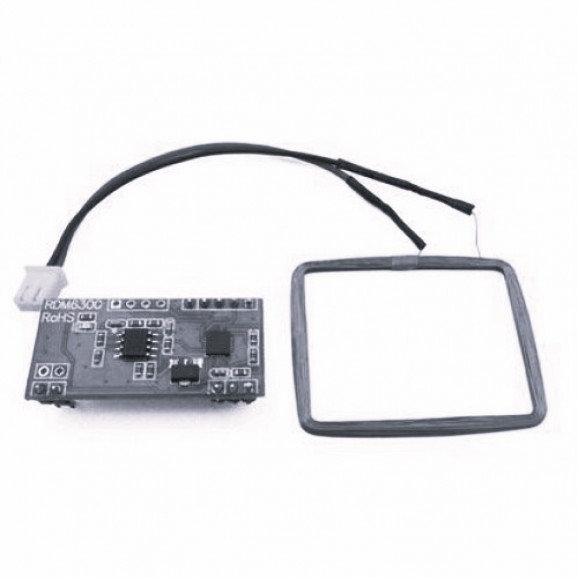
\includegraphics[width=0.5\linewidth]{img/rdm6300.jpg}
    \caption{Leitor RFID RDM6300.}
    \label{fig:RDM6300}
\end{figure}

\section{Configuração no ESP32 e no RFID}

O que foi usado na prática foi um ESP32 de 30 pinos, uma protoboard de 400 pontos, um RFID RDM6300 com frequência de 125 kHz (os cartões do IFCE utilizam essa frequência para troca de dados), três cabos fêmea-fêmea, dois cabos macho-fêmea e um cabo microUSB. RFID já vem conectado com uma ântena.

\begin{figure}[H]
    \centering
    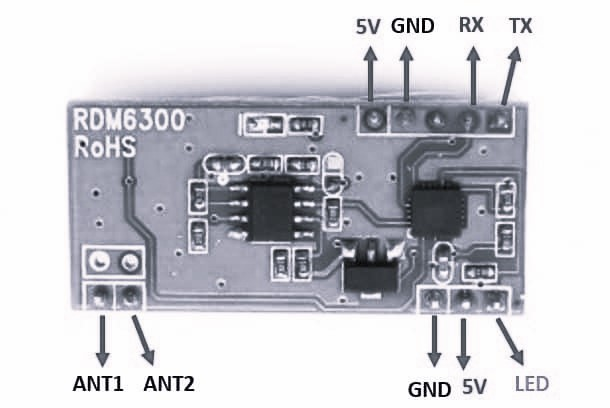
\includegraphics[width=0.5\linewidth]{img/RDM6300-RFID-pinout.jpg}
    \caption{Pinout do RDM6300.}
    \label{fig:RDM6300-pinout}
\end{figure}

Primeiro, providenciamos a fonte de alimentação para o RFID que vai vir do ESP32. Conectamos do pino 5V do leitor ao pino VIN do ESP32 que fornece exatamente 5V. Utilizamos um cabo fêmea-fêmea para conectar diretamente sem utilizar a protoboard.

Para que ocorra troca de dados entre ESP32 e o RFID, conectamos o pino RX de um ao TX do outro e vice-versa. Utilizamos cabos fêmea-fêmea e novamente fizemos a ligação sem a protoboard. Por padrão, os pinos de transferência de dados do ESP32 são os pinos 1 e 3 que são respectivamente o TX0 e o RX0. Caso queira outros, é preciso configurar em código, mas permanecemos no padrão.

\begin{figure}[H]
    \centering
    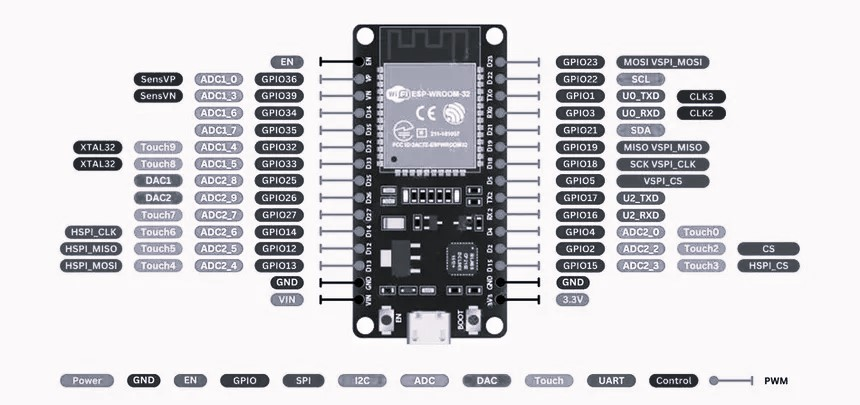
\includegraphics[width=0.5\linewidth]{img/esp32_pinout.png}
    \caption{Pinout do ESP32 de 30 pinos.}
    \label{fig:esp32-pinout}
\end{figure}

O ESP32 e o RFID precisam ter um GND de referência. Por isso, utilizamos dois cabos macho-fêmea para conectar os dois dispositivos na mesma coluna na protoboard.

O RFID RDM6300 possui dois pinos para a alimentação e dois pinos para o GND. Utilizamos os pinos que são vizinhos aos pinos de RX e TX, mas os pinos ao lado do LED também poderiam ser usados.

\begin{figure}[H]
    \centering
    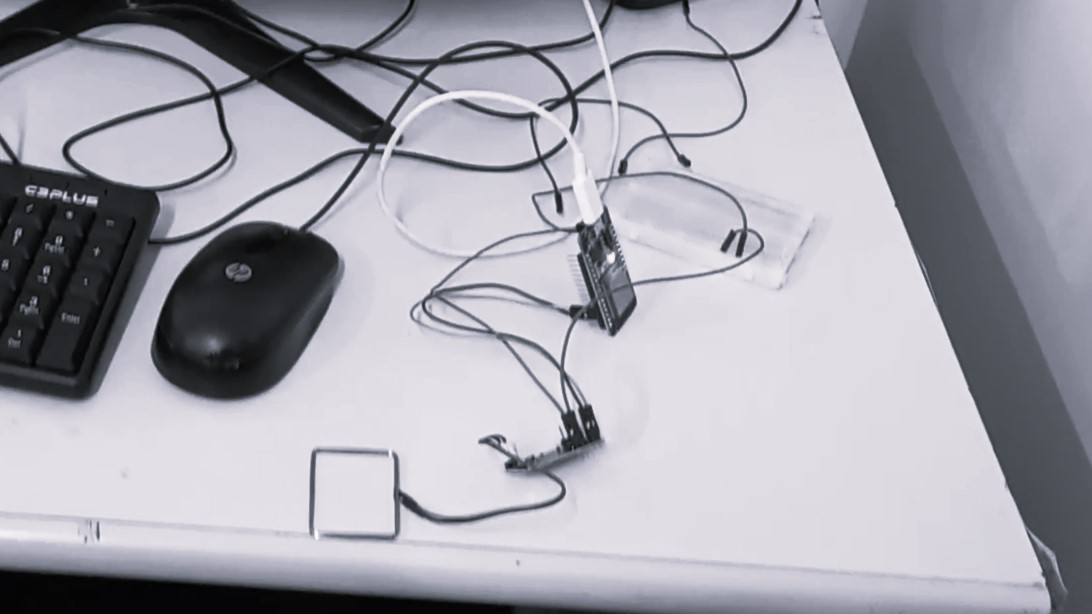
\includegraphics[width=0.5\linewidth]{img/final-config.jpg}
    \caption{Configuração final.}
    \label{fig:final-config}
\end{figure}

\section{Desenvolvimento do Código}

O desenvolvimento do código para imprimir o texto do cartão é bem simples devido a não precisar de bibliotecas além da biblioteca do Arduino. Abrimos a tela inicial do PlatformIO no VSCode e criamos um novo projeto chamado \textit{leitura\_cartao} com a placa \textit{Espressif ESP32 Dev Module} e o framework \textit{Arduino}.

\lstinputlisting[language=C++, firstline=3, lastline=3]{code/main.cpp}

Antes, criamos uma variável do tipo String chamada cardCode que irá guardar o código do cartão. E na função setup, iniciamos a Serial com a taxa 9600. É obrigatório colocar especificamente essa taxa para que os valores apareçam no monitor. Também precisamos definir essa taxa no arquivo \textit{platformio.ini} que é o arquivo de configuração que fica na raiz do projeto. Adicionamos \textit{monitor\_speed = 9600}.

\begin{lstlisting}
// main.cpp
void setup() {
    Serial.begin(9600)
}

// platformio.ini
monitorspeed = 9600

\end{lstlisting}

O resto da imprementação acontece apenas na função loop. Nela, criamos uma laço while que a sua condição é se existe dados no buffer serial ou não. Para conferir se existe alguma coisa no buffer, usamos o método \textit{available}. Ele mudará de estado quando passarmos o cartão na antena.

Entrando no laço de repetição, iremos guardar cada caractere que está no buffer e concatenar com a String cardCode. No início de cada iteração, utilizamos o método read do Serial para ler um caractere e guardar numa variável do tipo \textit{char} chamada de incomingChar. Logo após, concatenamos com cardCode utilizando o operador \textit{+=}, que funciona para concatenar strings.

\lstinputlisting[language=C++, firstline=15, lastline=17]{code/main.cpp} 

\lstinputlisting[language=C++, firstline=25, lastline=25]{code/main.cpp}

Para encerrar, criamos uma forma do fluxo sair do laço quando chegar ao fim dos dados do buffer. O professor informou que o último byte do buffer possui valor 0x03, justamente para indicar que aquele é o final. Então, utilizamos um if condicional para compar se o valor de incomingChar dessa iteração é igual à 0x03. Se for, antes de usarmos um \textit{break} para sair do \textit{while}, iremos imprimir o conteúdo de \textit{cardCode} para logo depois apagarmos o conteúdo para a próxima leitura.

\lstinputlisting[language=C++, firstline=18, lastline=22]{code/main.cpp}

O motivo de não confiarmos apenas no \textit{available} do Serial deixar de ser positivo para que ele saia do \textit{while} é que a condição não é instantânea. Podendo ocorrer do código do cartão ser escrito mais de uma vez em \textit{carCode}.

É possível conferir o código completo nesse \href{https://github.com/fabricio-araujo94/microcontroladores/tree/main/leitura_cartao}{repositório} no GitHub.

\section{Considerações Finais}

Feito tudo isso, conectamos o ESP32 ao computador utilizando o cabo microUSB. Antes de fazermos \textit{upload} no código, removemos os cabos dos pinos de RX e TX do ESP32. Só depois do código ter sido carregado que conectamos o cabo aos pinos. Acontece que os pinos RX0 e TX0 são usados normalmente para a comunição com o monitor serial, mas eles podem ser usados para se conectar com outros dispositos depois que o código já foi recebido.

Depois de conectado, apertamos o botão de boot do ESP32 apenas por precaução. Agora, passamos o cartão de acesso do IFCE na antena do RFID e o código do cartão aparece no monitor.

O funcionamento da prática pode ser vista nesse \href{https://youtu.be/eZHZmrigDyo}{vídeo} no YouTube.

\end{document}